\subsection{Parameter Effects}
\label{sec:setup.char.paramfx}

This section is concerned with the other types of characteristics, the effects of the parameters of the model on the shape of the model function.
First, it analyzes the combined parameter effects along a chain of parameter regions assocoated with cycles the same period.
After that, it analyzes the isolated effects of the single parameters and decomposes the combined effects into the isolated effects.

\subsection{Combined Effects of Parameters}
\label{sec:setup.char.paramfx.combined}

To replicate the dynamics seen in the model, it is helpful to know, how the model changes along the chains of parameter regions that are associated with cycles of the same period.
This section therefore analyzes the model function at different points in different chains.
\Cref{fig:setup.char.evolution.map} indicates the points used for this analysis.
\Cref{fig:setup.char.evolution.12} shows, how the model function changes along the chain of parameter regions associated with cycles of period 12.
In the figure, there are three functions $F^{A_12}, F^{B_12},$ and $F^{C_12}$.
The function $F^{A_{12}}$ is the model function with the parameters $E_0 = 15.9, \chi_0 = 0.11$.
These parameter values are marked with the point $A_{12}$ in \Cref{fig:setup.char.evolution.map}.
The function $F^{B_{12}}$ is the model function with the parameters $E_0 = 17.07, \chi_0 = 0.182$.
And the function $F^{C_{12}}$ is the model function with the parameters $E_0 = 18.5, \chi_0 = 0.27$.
The parameter values are marked accordingly in \Cref{fig:setup.char.evolution.map}.

\begin{figure}
	\centering
	\subfloat[Points]{
		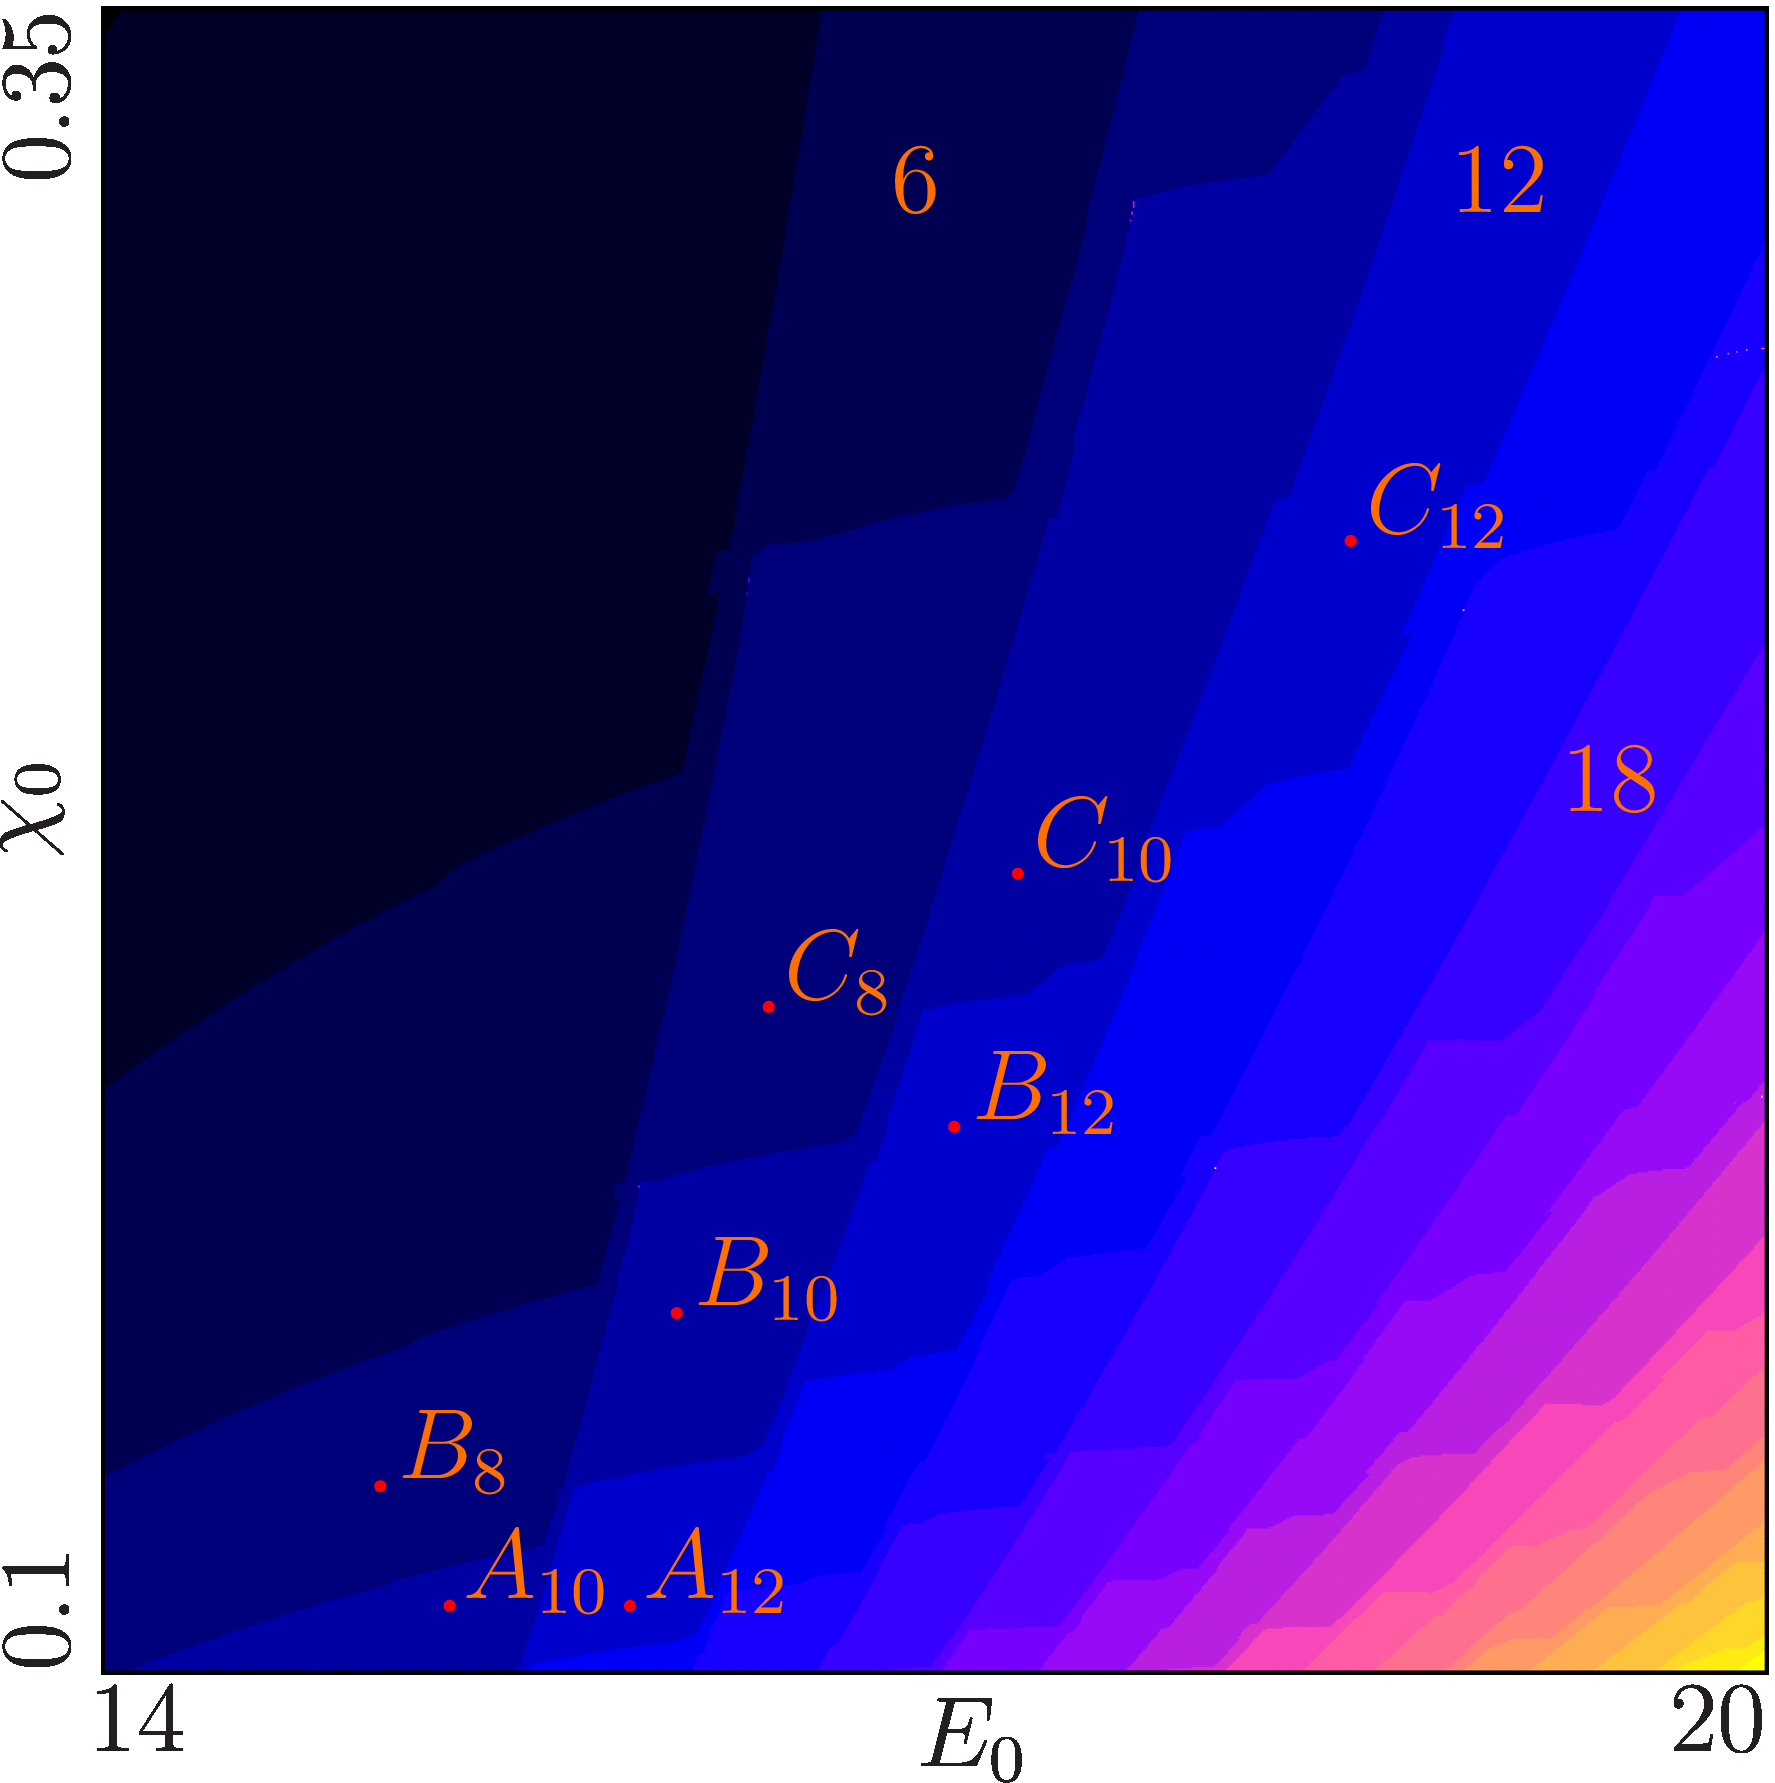
\includegraphics[width=.4 \textwidth]{../Figures/5/5.2a/result.png}
		\label{fig:setup.char.evolution.map}
	}
	\subfloat[Period $12$]{
		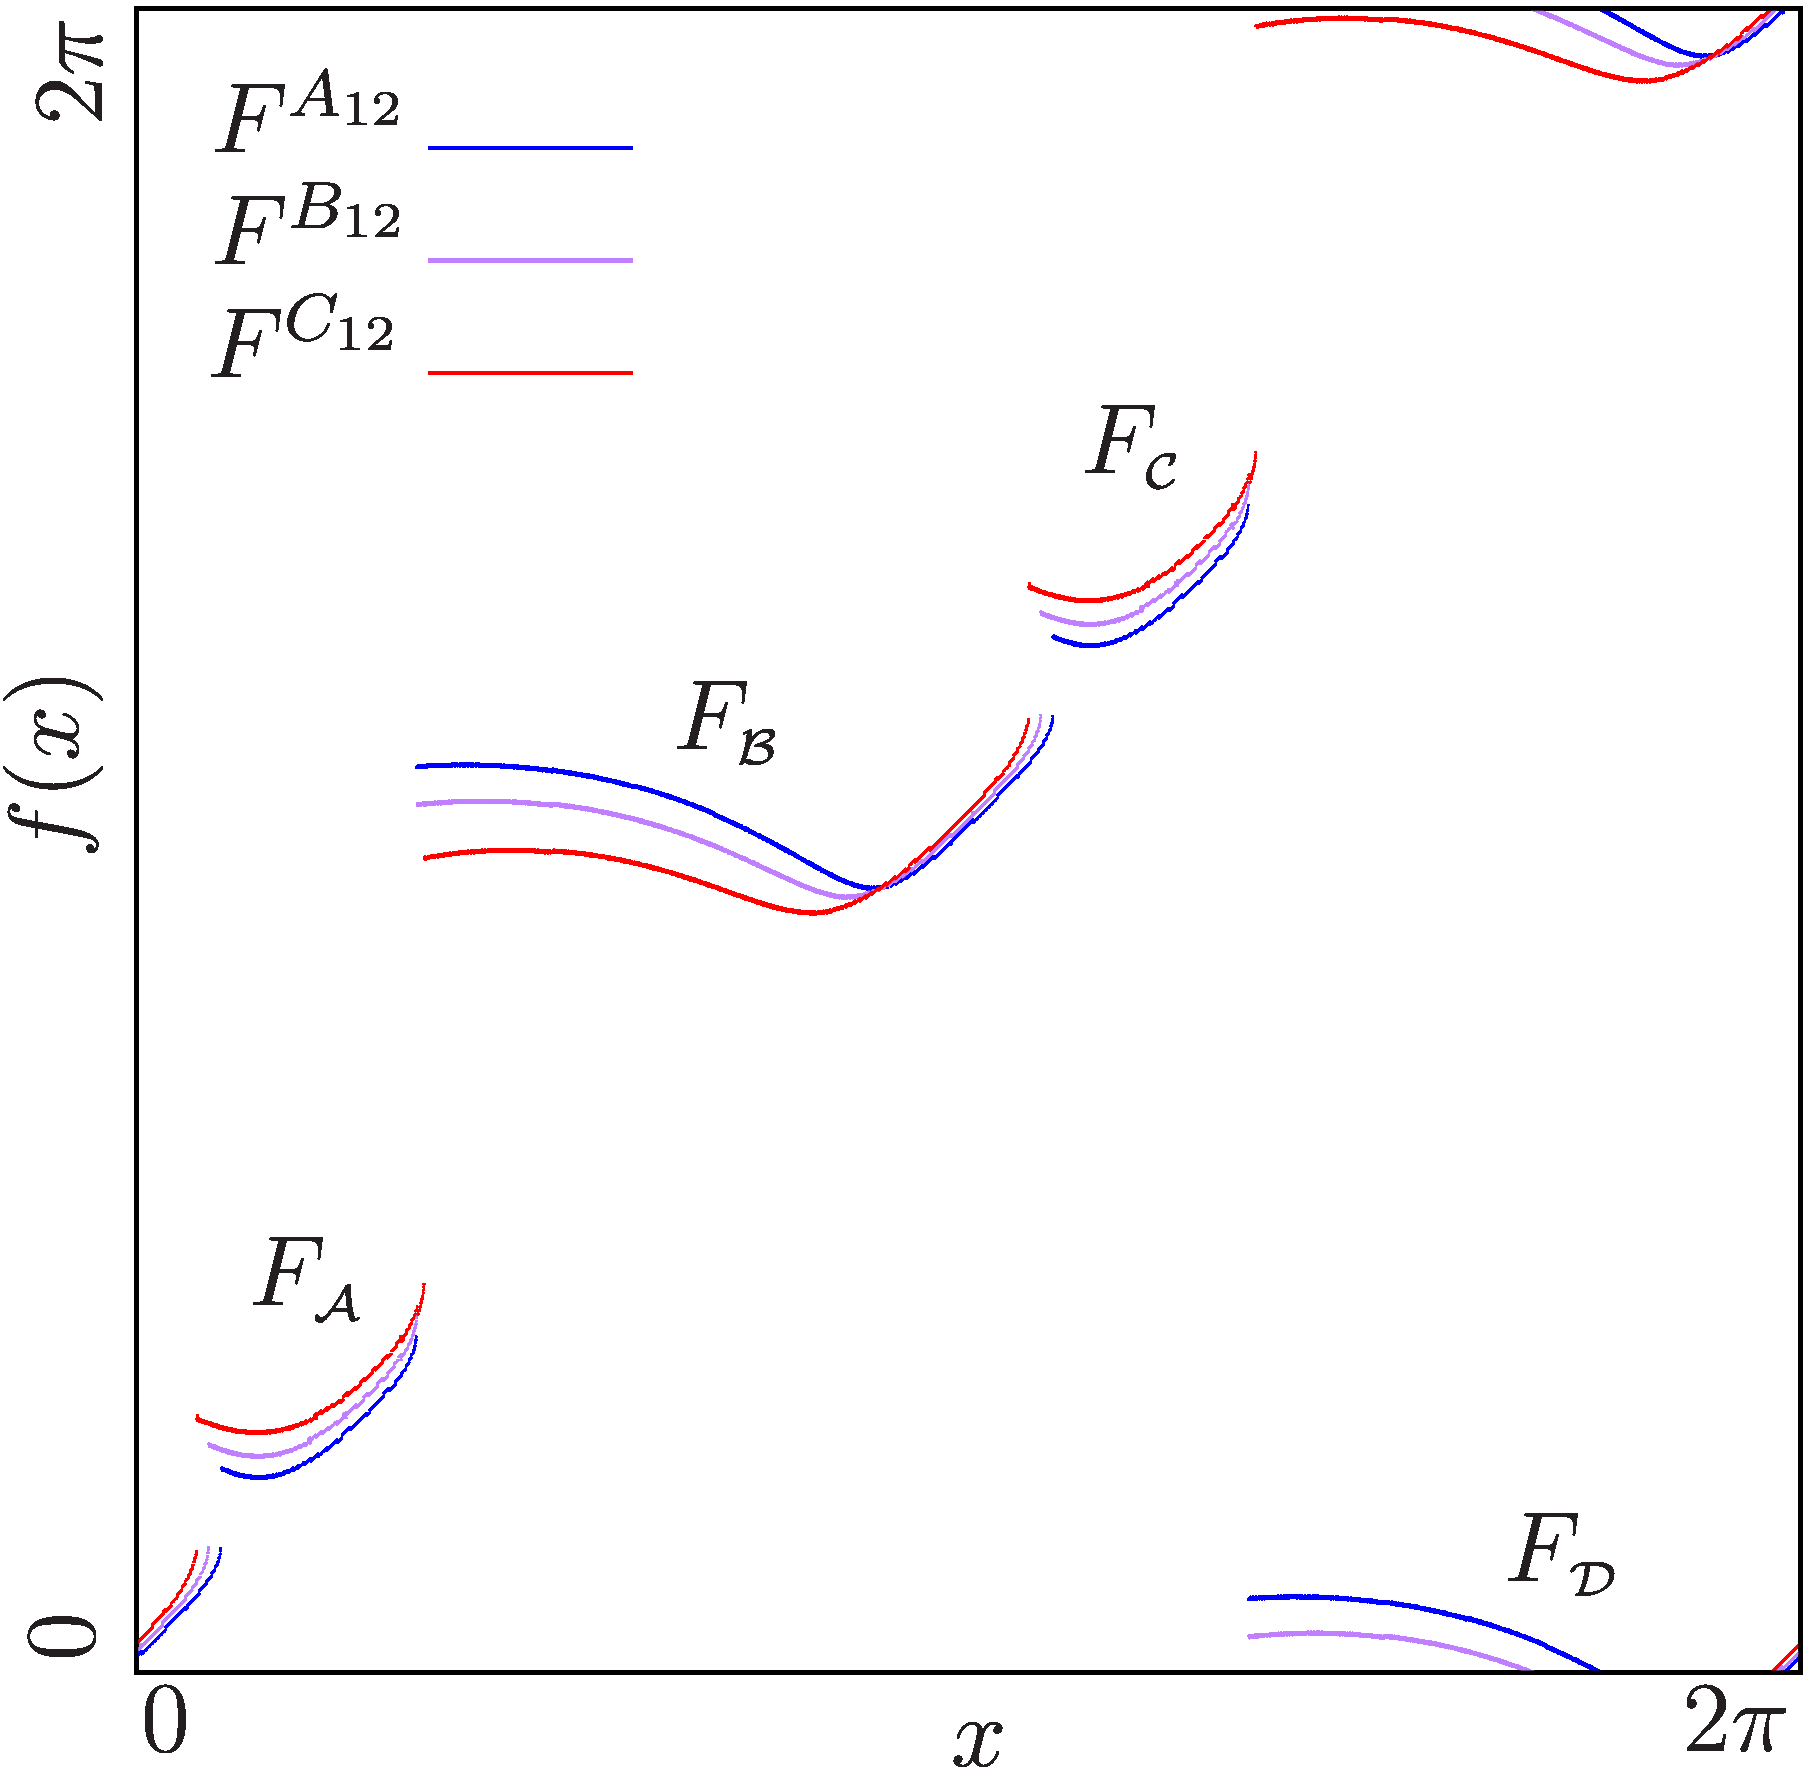
\includegraphics[width=.4 \textwidth]{../Figures/5/5.2b/illustration.png}
		\label{fig:setup.char.evolution.12}
	} \\
	\subfloat[Period $10$]{
		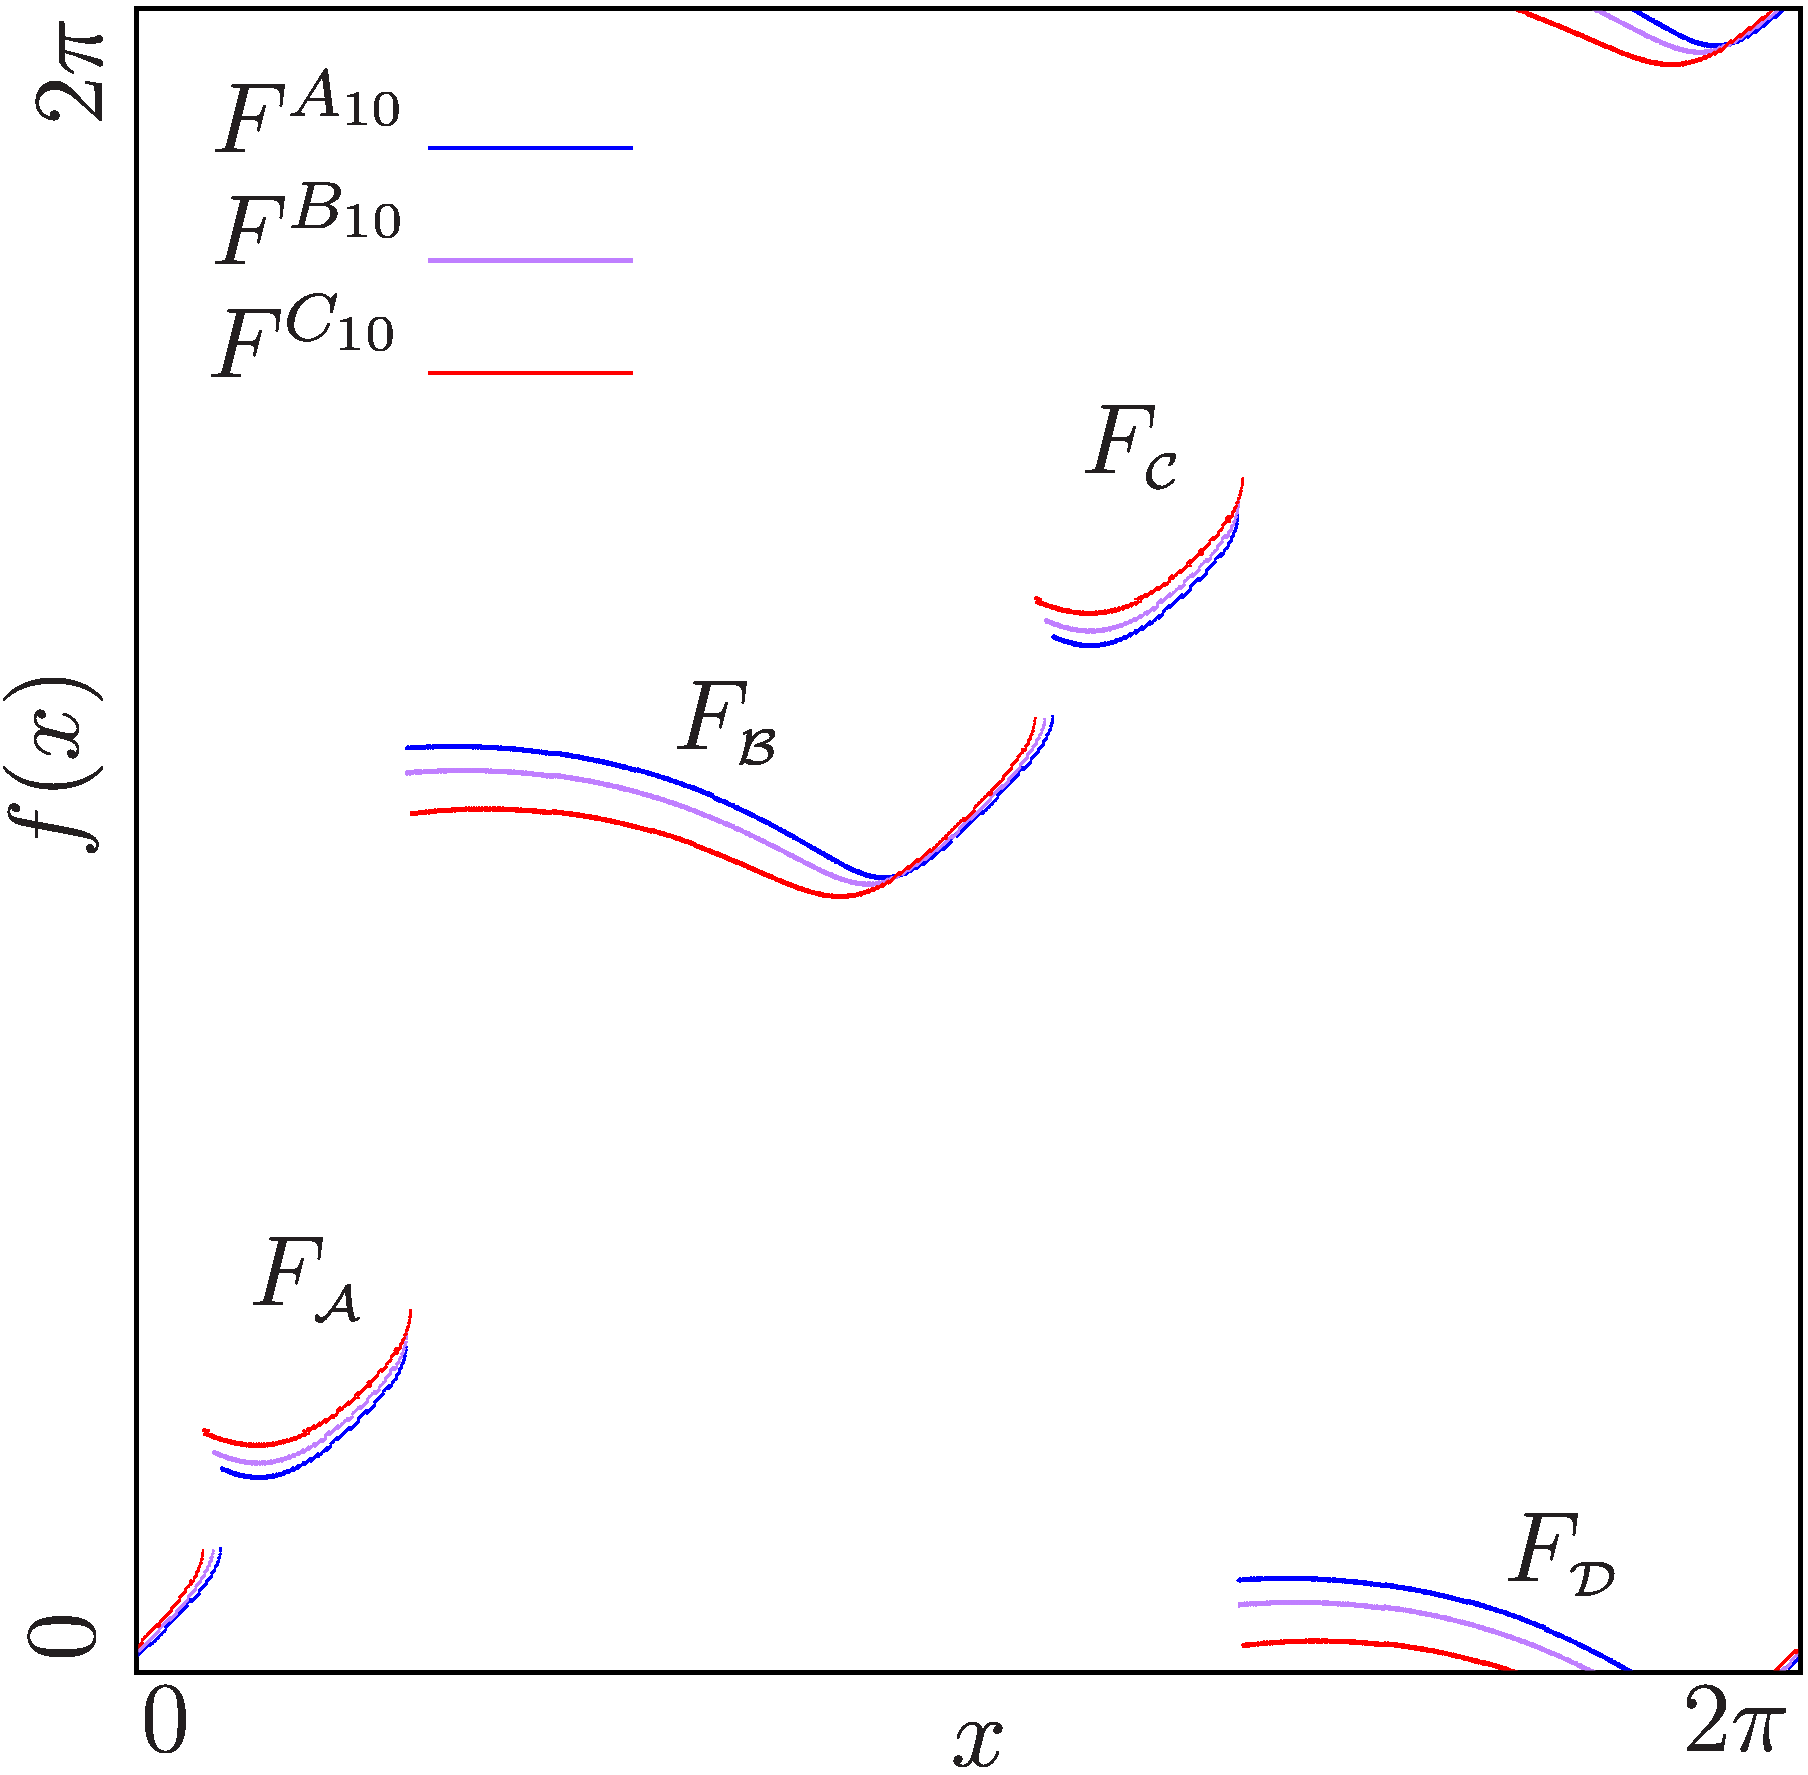
\includegraphics[width=.4 \textwidth]{../Figures/5/5.2c/illustration.png}
		\label{fig:setup.char.evolution.10}
	}
	\subfloat[Period $8$]{
		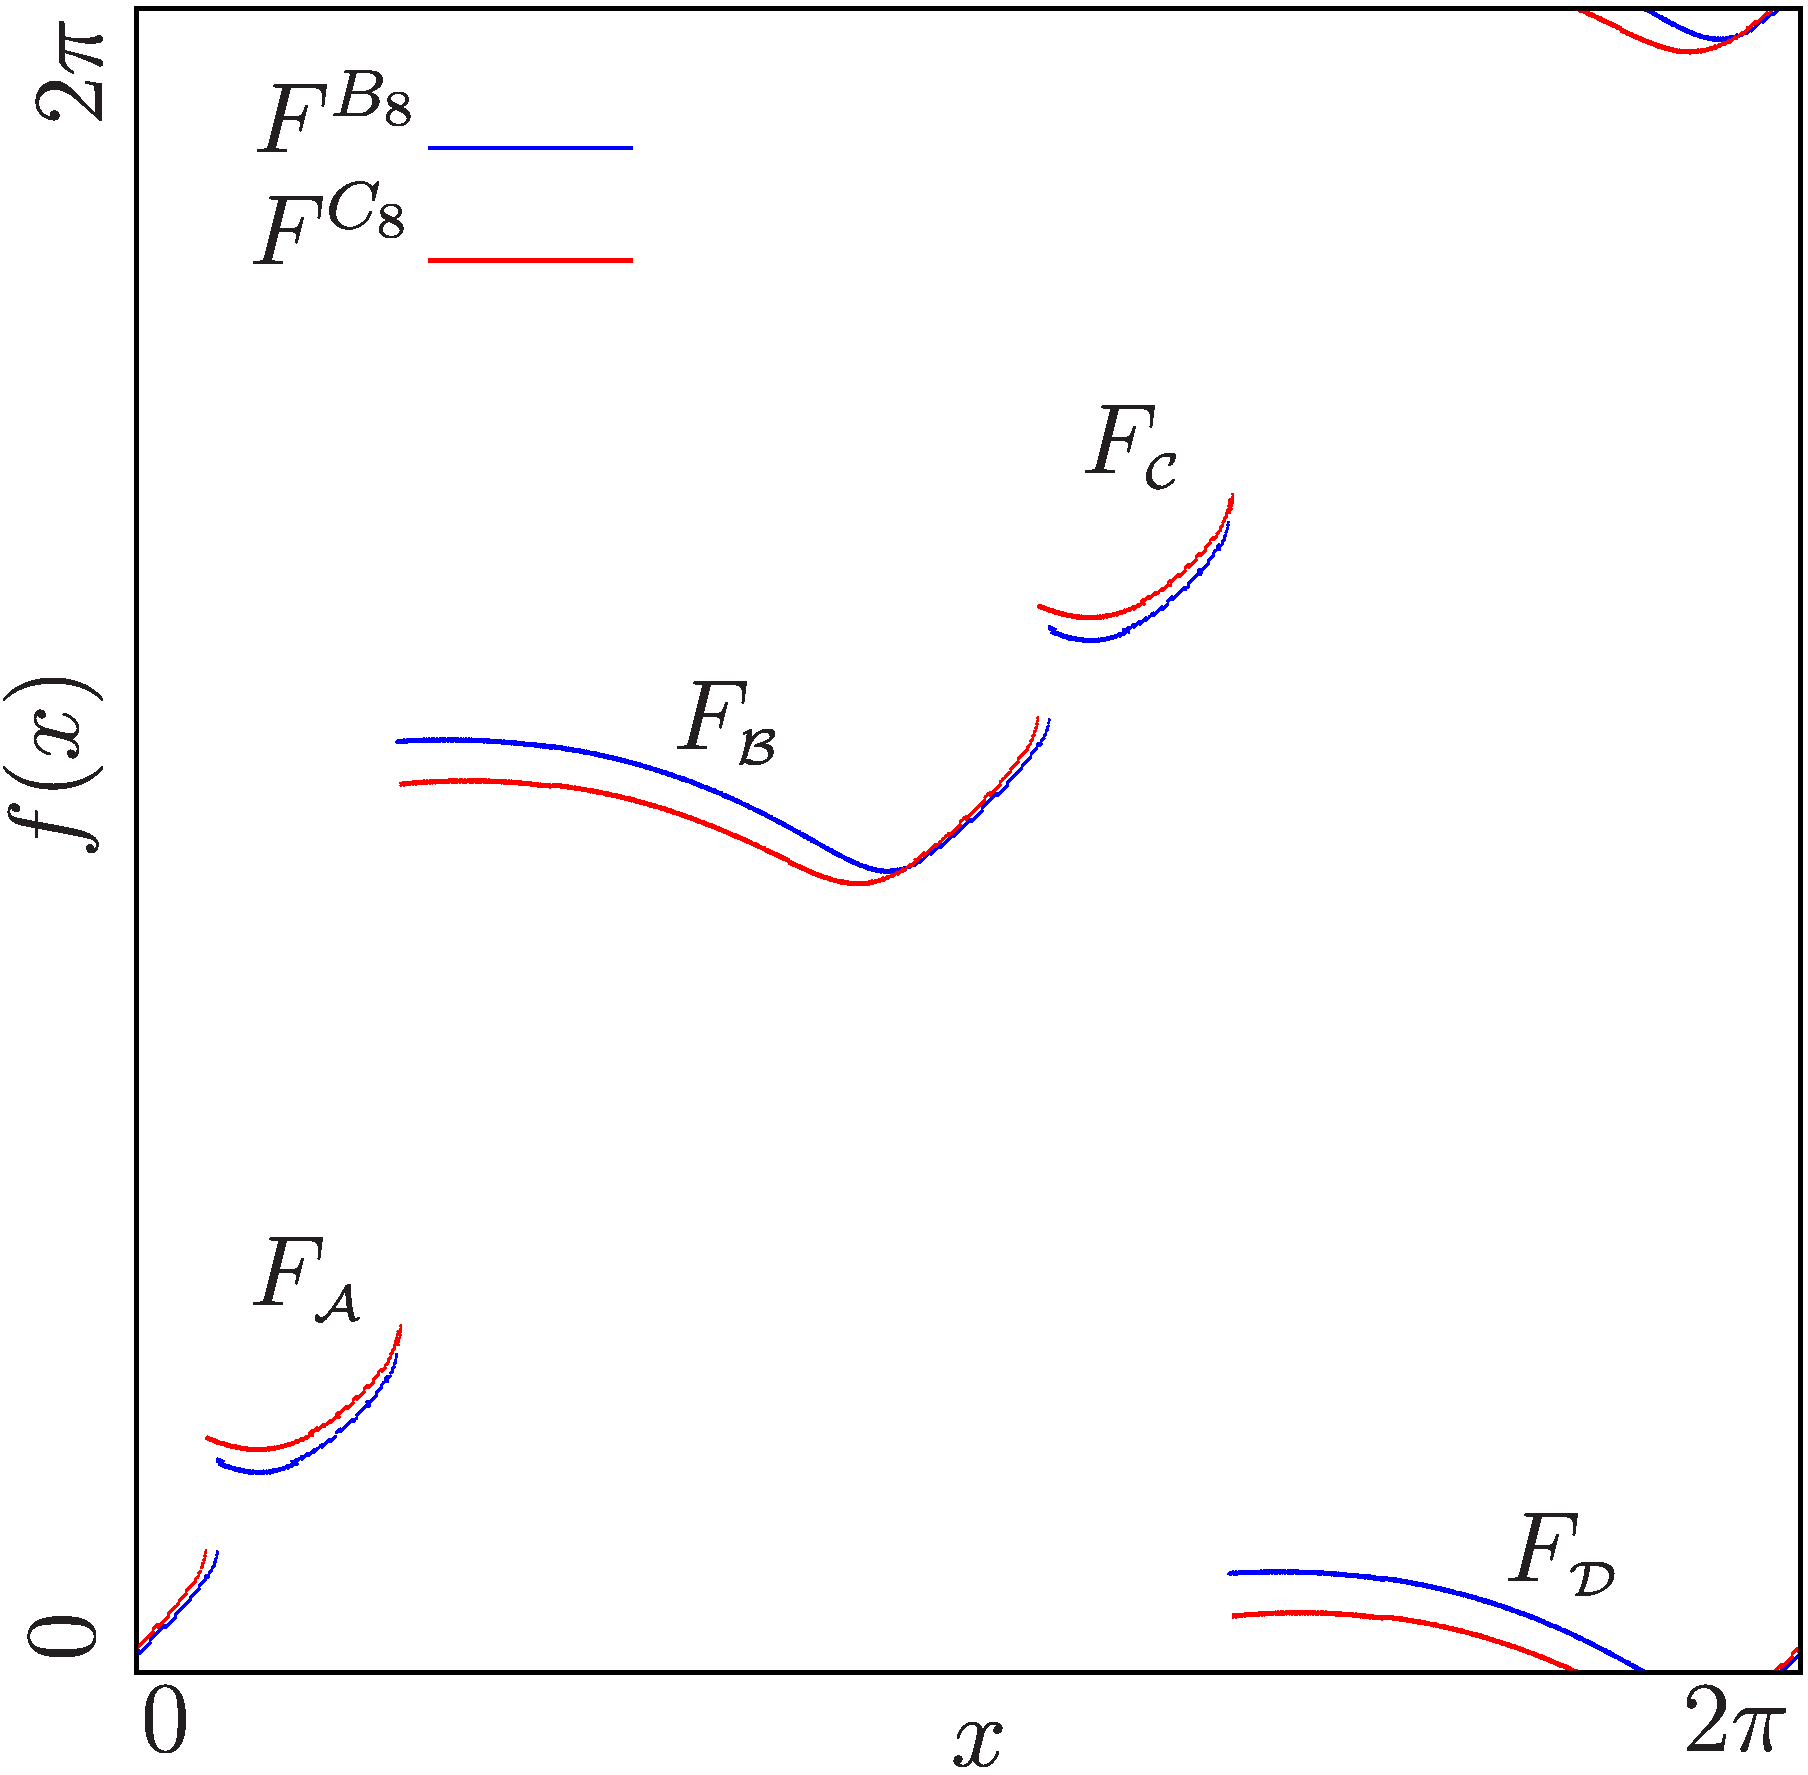
\includegraphics[width=.4 \textwidth]{../Figures/5/5.2d/illustration.png}
		\label{fig:setup.char.evolution.08}
	}
	\caption[The effects of the parameters on the original model function]{
		The effects of the parameters on the original model function illustrated by plotting the model function at different parameter values.
		The parameters $\beta = 1, f = 150, L = 4.2 \cdot 10^{-3}, R = 2, V_m = 5,$ and $\mu = 0.5$ are fixed.
		(a) shows a 2D scan of the periods associated with parameter regions in the original model.
		The parameters $E_0$ and $\chi_0$ are varied in the ranges $[14, 20]$ and $[0.1, 0.35]$.
		The points in this scan mark the parameter values used for plotting the model function in (b), (c), and (d).
		(b) shows the evolution of the shape of the model function along the chain of parameter regions associated with the period 12.
		The function $F^{A_{12}}$ is the model function with the parameter values at the point $A_{12}$ where $E_0 = 15.9$ and $\chi_0 = 0.11$,
		$F^{B_{12}}$ at the point $B_{12}$ where $E_0 = 17.07$ and $\chi_0 = 0.182$,
		and $F^{C_{12}}$ at the point $C_{12}$ where $E_0 = 18.5$ and $\chi_0 = 0.27$.
		(c) shows the evolution of the shape of the model function along the chain of parameter regions associated with the period 10.
		Here, $F^{A_{10}}$ is the model function with the parameters at the point $A_{10}$ where $E_0 = 15.25$ and $\chi_0 = 0.11$,
		$F^{B_{10}}$ at the point $B_{10}$ where $E_0 = 16.07$ and $\chi_0 = 0.154$,
		and $F^{C_{10}}$ at the point $C_{10}$ where $E_0 = 17.3$ and $\chi_0 = 0.22$.
		And (d) shows the evolution of the shape of the model function along the chain of parameter regions associated with the period 8.
		Here, $F^{B_8}$ is the model function with the parameter values at the point $B_8$ where $E_0 = 15$ and $\chi_0 = 0.128$,
		and $F^{C_8}$ at the point $C_8$ where $E_0 = 16.4$ and $\chi_0 = 0.2$.
	}
	\label{fig:setup.char.evolution.combined}
\end{figure}

The most notable changes are the following.
\begin{enumerate}
	\item The values of the whole branches $F_\A$ and $F_\C$ get larger.
	      This change is most notable at the left borders of the branches.
	      The values on the left sides of the branches are affected more by this change than the values on the right sides.
	\item The values on the left sides of the branches $F_\B$ and $F_\D$ get smaller while the values on the right sides are not affected much.
	\item The local minima of the branches $F_\B$ and $F_\D$ move to the left, and their values get smaller.
\end{enumerate}
One smaller change is that the border between branches $F_\B$ and $F_\C$ moves left.
Note that the same change happens to the border between the branches $F_\D$ and $F_\A$ due to the symmetry of the function.

The same effects can be observed in the chains of parameter regions associated with cycles of periods $10$ and $8$, respectively.
For the chain of parameter regions associated with cycles of period $10$, the model function is plotted in \Cref{fig:setup.char.evolution.10} at the three points $A_{10}, B_{10},$ and $C_{10}$ marked in \Cref{fig:setup.char.evolution.map}.
Again, the values of the whole branches $F_\A$ and $F_\C$ are larger in $F^{C_{10}}$ than they are in $F^{A_{10}}$.
And the values on the left sides of the branches $F_\B$ and $F_\D$ are smaller in $F^{C_{10}}$ than they are in $F^{A_{10}}$.
Also, the local minima on those branches move left and down.
For the chain of parameter regions associated with cycles of period $8$, the model function is plotted in \Cref{fig:setup.char.evolution.08} at the two points $B_8$ and $C_8$ marked in \Cref{fig:setup.char.evolution.map}.
And the values of the branches undergo the same changes again from the model function $F^{B_8}$ to $F^{C_8}$.

\subsection{Individual Effects of Parameters}
\label{sec:setup.char.paramfx.individual}

The effects of the parameters described above, always include a change in both parameters $E_0$ and $\chi_0$.
To reproduce the bifurcation structures, it is important to know which effects on the function each parameter has individually.
This section focuses on the isolated effects of each parameter by fixing one of the parameters and only varying the other one and observing the effects of this parameter on the shape of the model function.

\begin{figure}
	\centering
	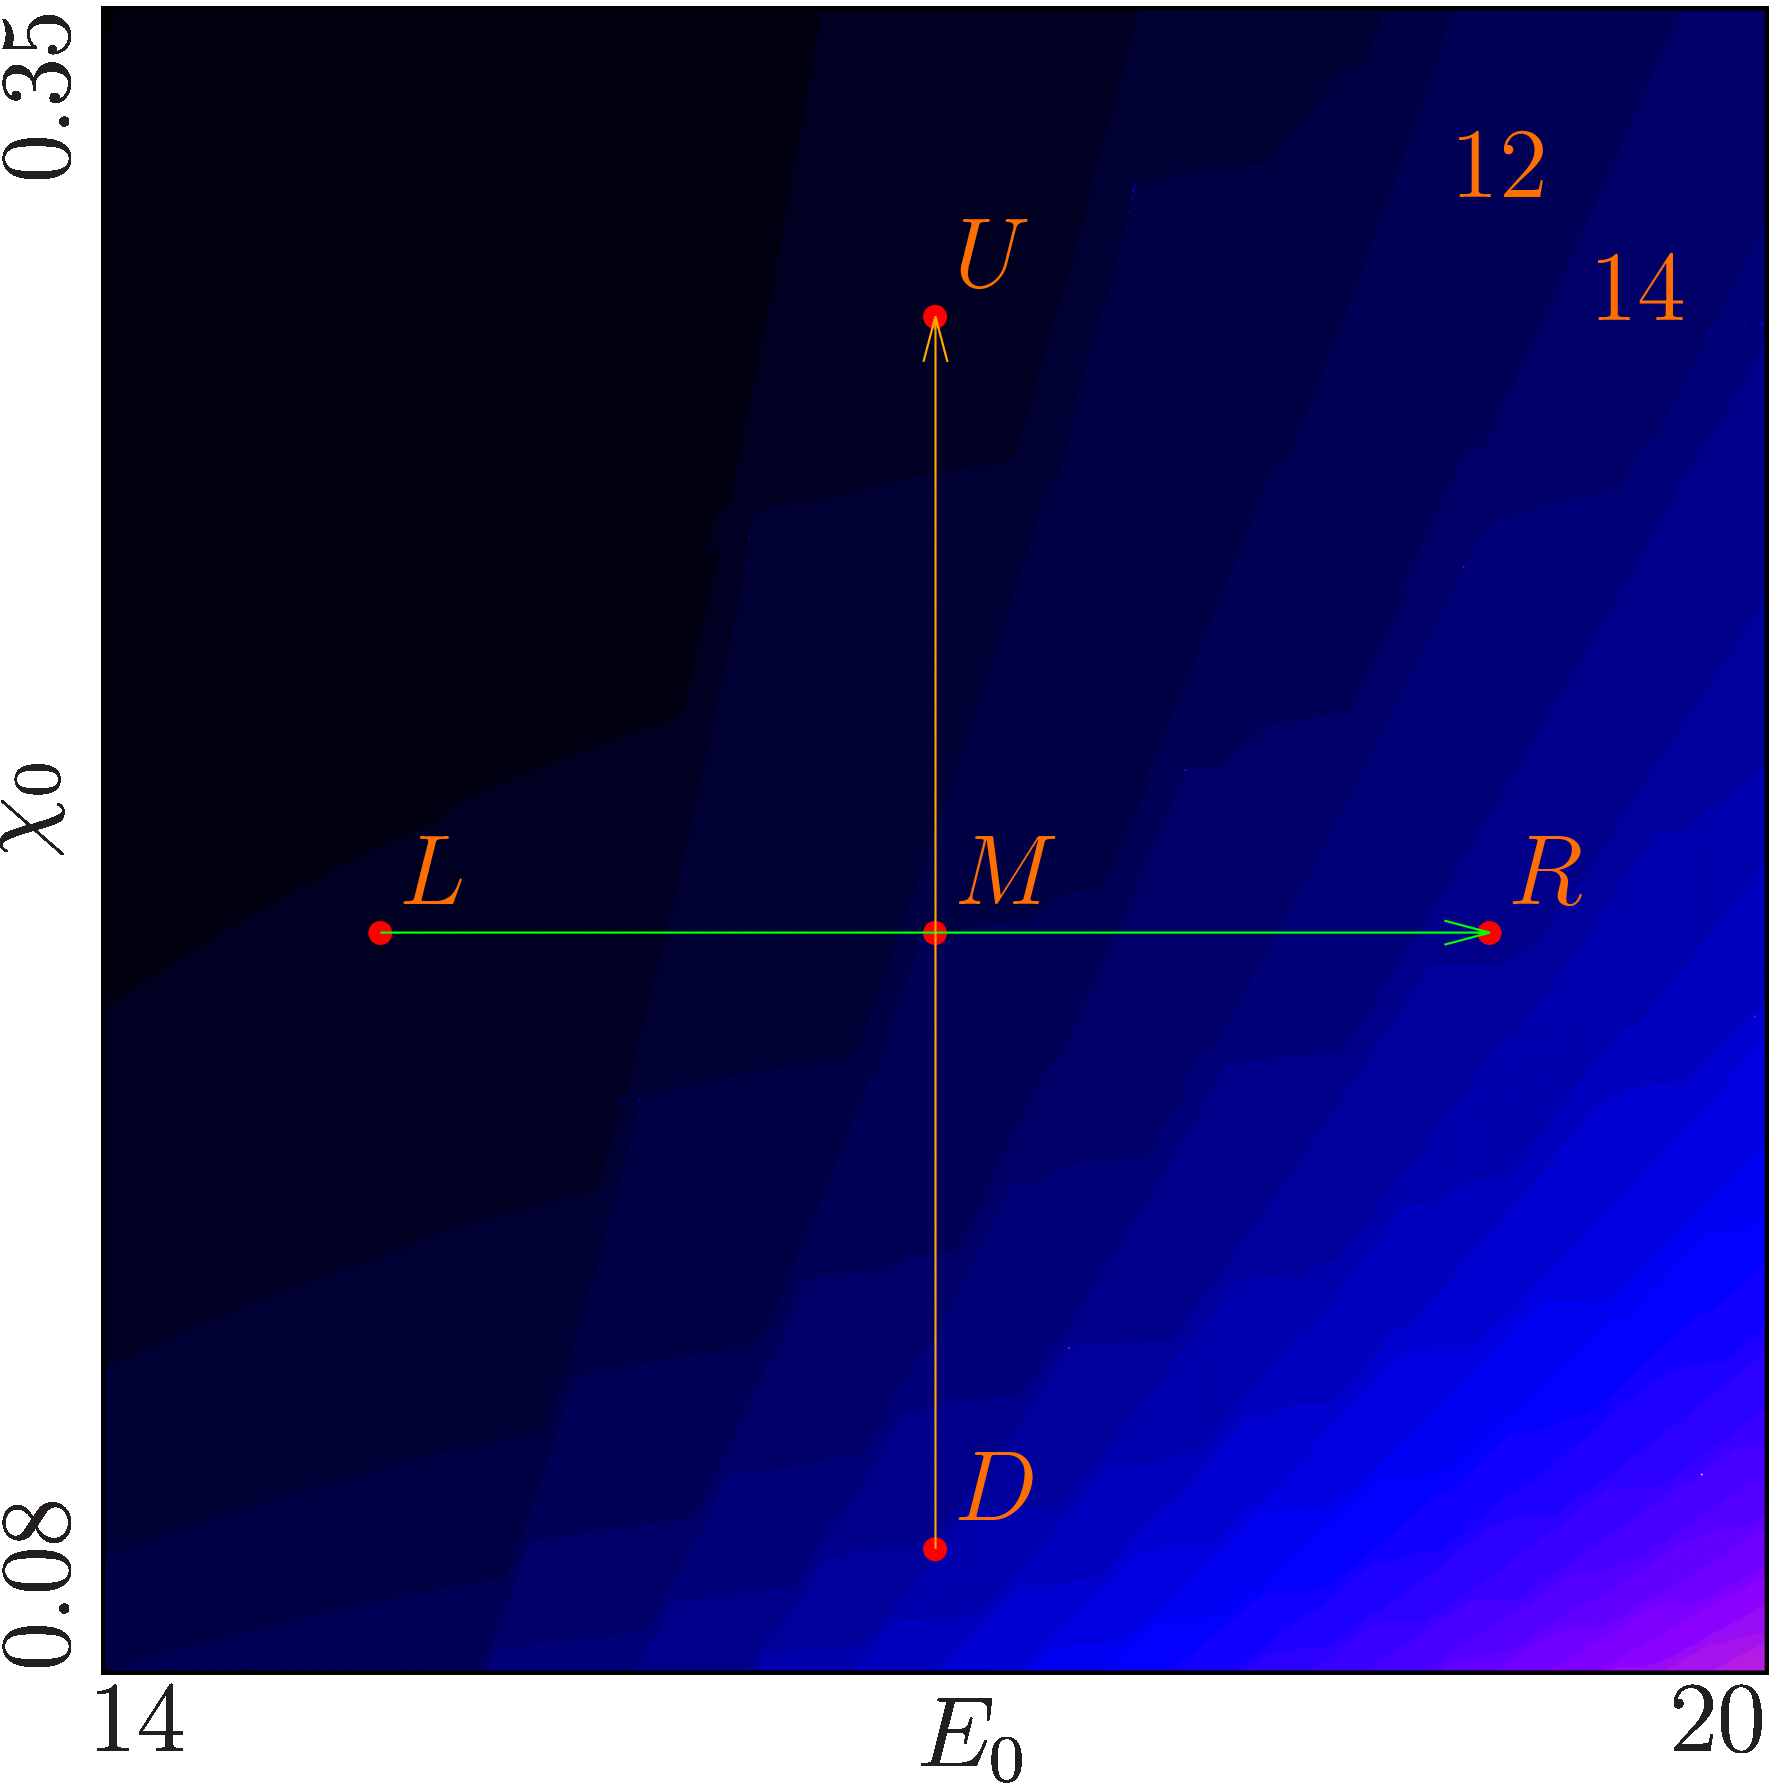
\includegraphics[width=0.4\textwidth]{../Figures/5/5.3/result.png}
	\caption[The parameter ranges examined to analyze the isolated effects of parameters on the original model function]{
		2D scan of the periods associated with parameter regions in the original model.
		The parameters $\beta = 1, f = 150, L = 4.2 \cdot 10^{-3}, R = 2, V_m = 5,$ and $\mu = 0.5$ are fixed.
		The parameters $E_0$ and $\chi_0$ are varied in the ranges $[14, 20]$ and $[0.08, 0.35]$.
		It illustrates the parameter ranges used to analyze the isolated effects of the parameters $E_0$ and $\chi_0$ on the original model function.
		The green arrow indicates the parameter range used to analyze the effects of the parameter $E_0$, while the orange arrow indicates the parameter range used to analyze the effects of the parameter $\chi_0$ on the original model function.
		The points $L, M, R, D,$ and $U$ mark the parameter values used for the cobweb diagrams in \Cref{fig:setup.char.evolution.single}.
	}
	\label{fig:setup.char.evolution.single.map}
\end{figure}

For the effects of the parameter $E_0$, $\chi_0 = 0.2$ is fixed and $E_0$ is varied in the parameter range $[15, 19]$.
This is marked as the green arrow in \Cref{fig:setup.char.evolution.single.map}.
As before, the model function is plotted at three parameter values in one figure.
The functions are visualized in \Cref{fig:setup.char.evolution.e0}.
$F^L$ is the model function with $E_0 = 15$, $F^M$ is the model function with $E_0 = 17$, and $F^R$ is the model function with $E_0 = 17$.
$\chi_0 = 0.2$ is the same for all functions $F^L, F^M,$ and $F^R$.
The parameter values are marked with the points $L, M,$ and $R$ in \Cref{fig:setup.char.evolution.single.map}.
One can see that they are all on the green arrow mentioned before.
The following changes can be observed.
\begin{enumerate}
	\item The values on the left sides of the branches $F_\B$ and $F_\D$ get smaller while the values on the right sides are not affected much.	\item The local minima of the branches $F_\B$ and $F_\D$ move left, and their values get smaller.
	\item The border between the branches $F_\A$ and $F_\B$ moves to the right.
	      The same is true for the border between the branches $F_\C$ and $F_\D$ because of the symmetry in the original model.
	\item The values at the right borders of branches $F_\A$ and $F_\C$ get larger. This is caused by the border between branches $F_\A$ and $F_B$ moving to the right.
\end{enumerate}

For the effects of the parameter $\chi_0$, $E_0 = 17$ is fixed and $\chi_0$ is varied in the parameter range $[0.125, 0.3]$.
This parameter range is marked with an orange arrow in \Cref{fig:setup.char.evolution.single.map}.
Again, the model function is plotted at three parameter values in one figure.
The functions are visualized in \Cref{fig:setup.char.evolution.hi}.
$F^D$ is the model function with $\chi_0 = 0.1$, $F^M$ is the model function with $\chi_0 = 0.2$, and $F^U$ is the model function with $\chi_0 = 0.3$.
$E_0 = 15$ is the same for all functions $F^D, F^M,$ and $F^U$.
The parameter values are marked with the points $D, M,$ and $U$ in \Cref{fig:setup.char.evolution.single.map}.
One can see that they are all on the orange arrow mentioned before.
The following pronounced changes can be observed.
\begin{enumerate}
	\item The values of the whole branches $F_\A$ and $F_\C$ get larger.
	\item The border between the branches $F_\A$ and $F_\B$ moves to the left.
	      The same is true for the border between the branches $F_\C$ and $F_\D$.
\end{enumerate}
Two other smaller changes that can be observed are the following.
\begin{enumerate}
	\item The values on the right sides of the branches $F_\B$ and $F_\D$ get larger.
	      This includes the values of the local minima on these branches.
	\item The border between the branches $F_\B$ and $F_\C$ moves to the left.
	      The same is true for the border between the branches $F_\D$ and $F_\A$.
\end{enumerate}

\begin{figure}
	\centering
	\subfloat[$E_0$]{
		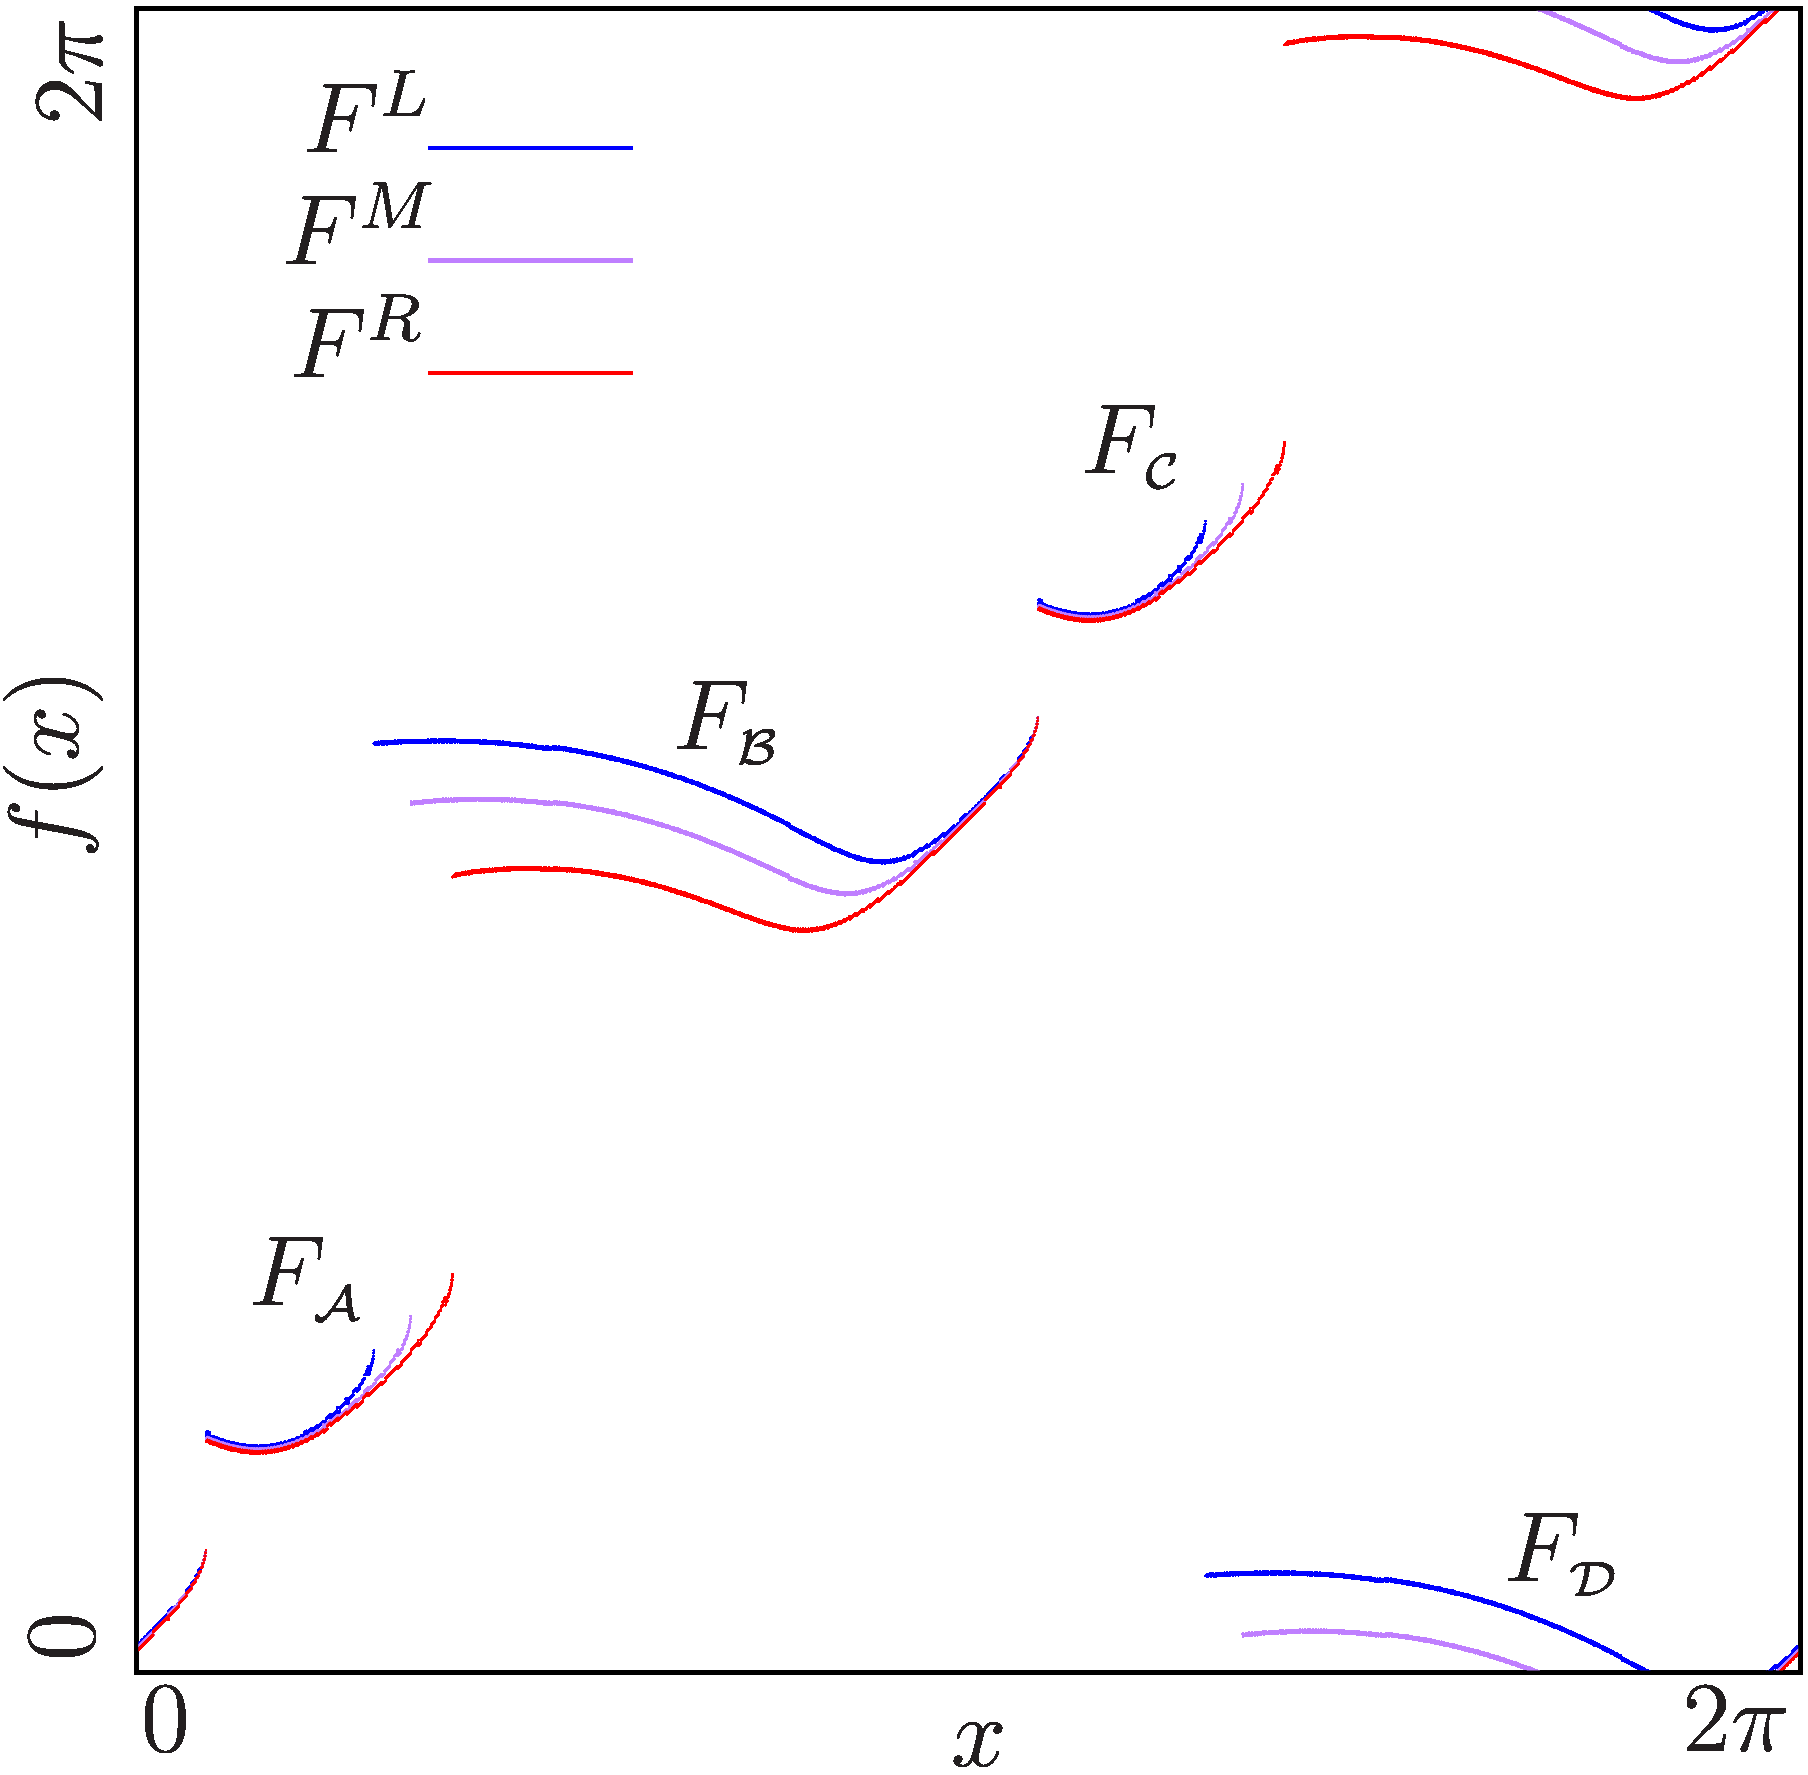
\includegraphics[width=.4 \textwidth]{../Figures/5/5.4a/illustration.png}
		\label{fig:setup.char.evolution.e0}
	}
	\subfloat[$\chi_0$]{
		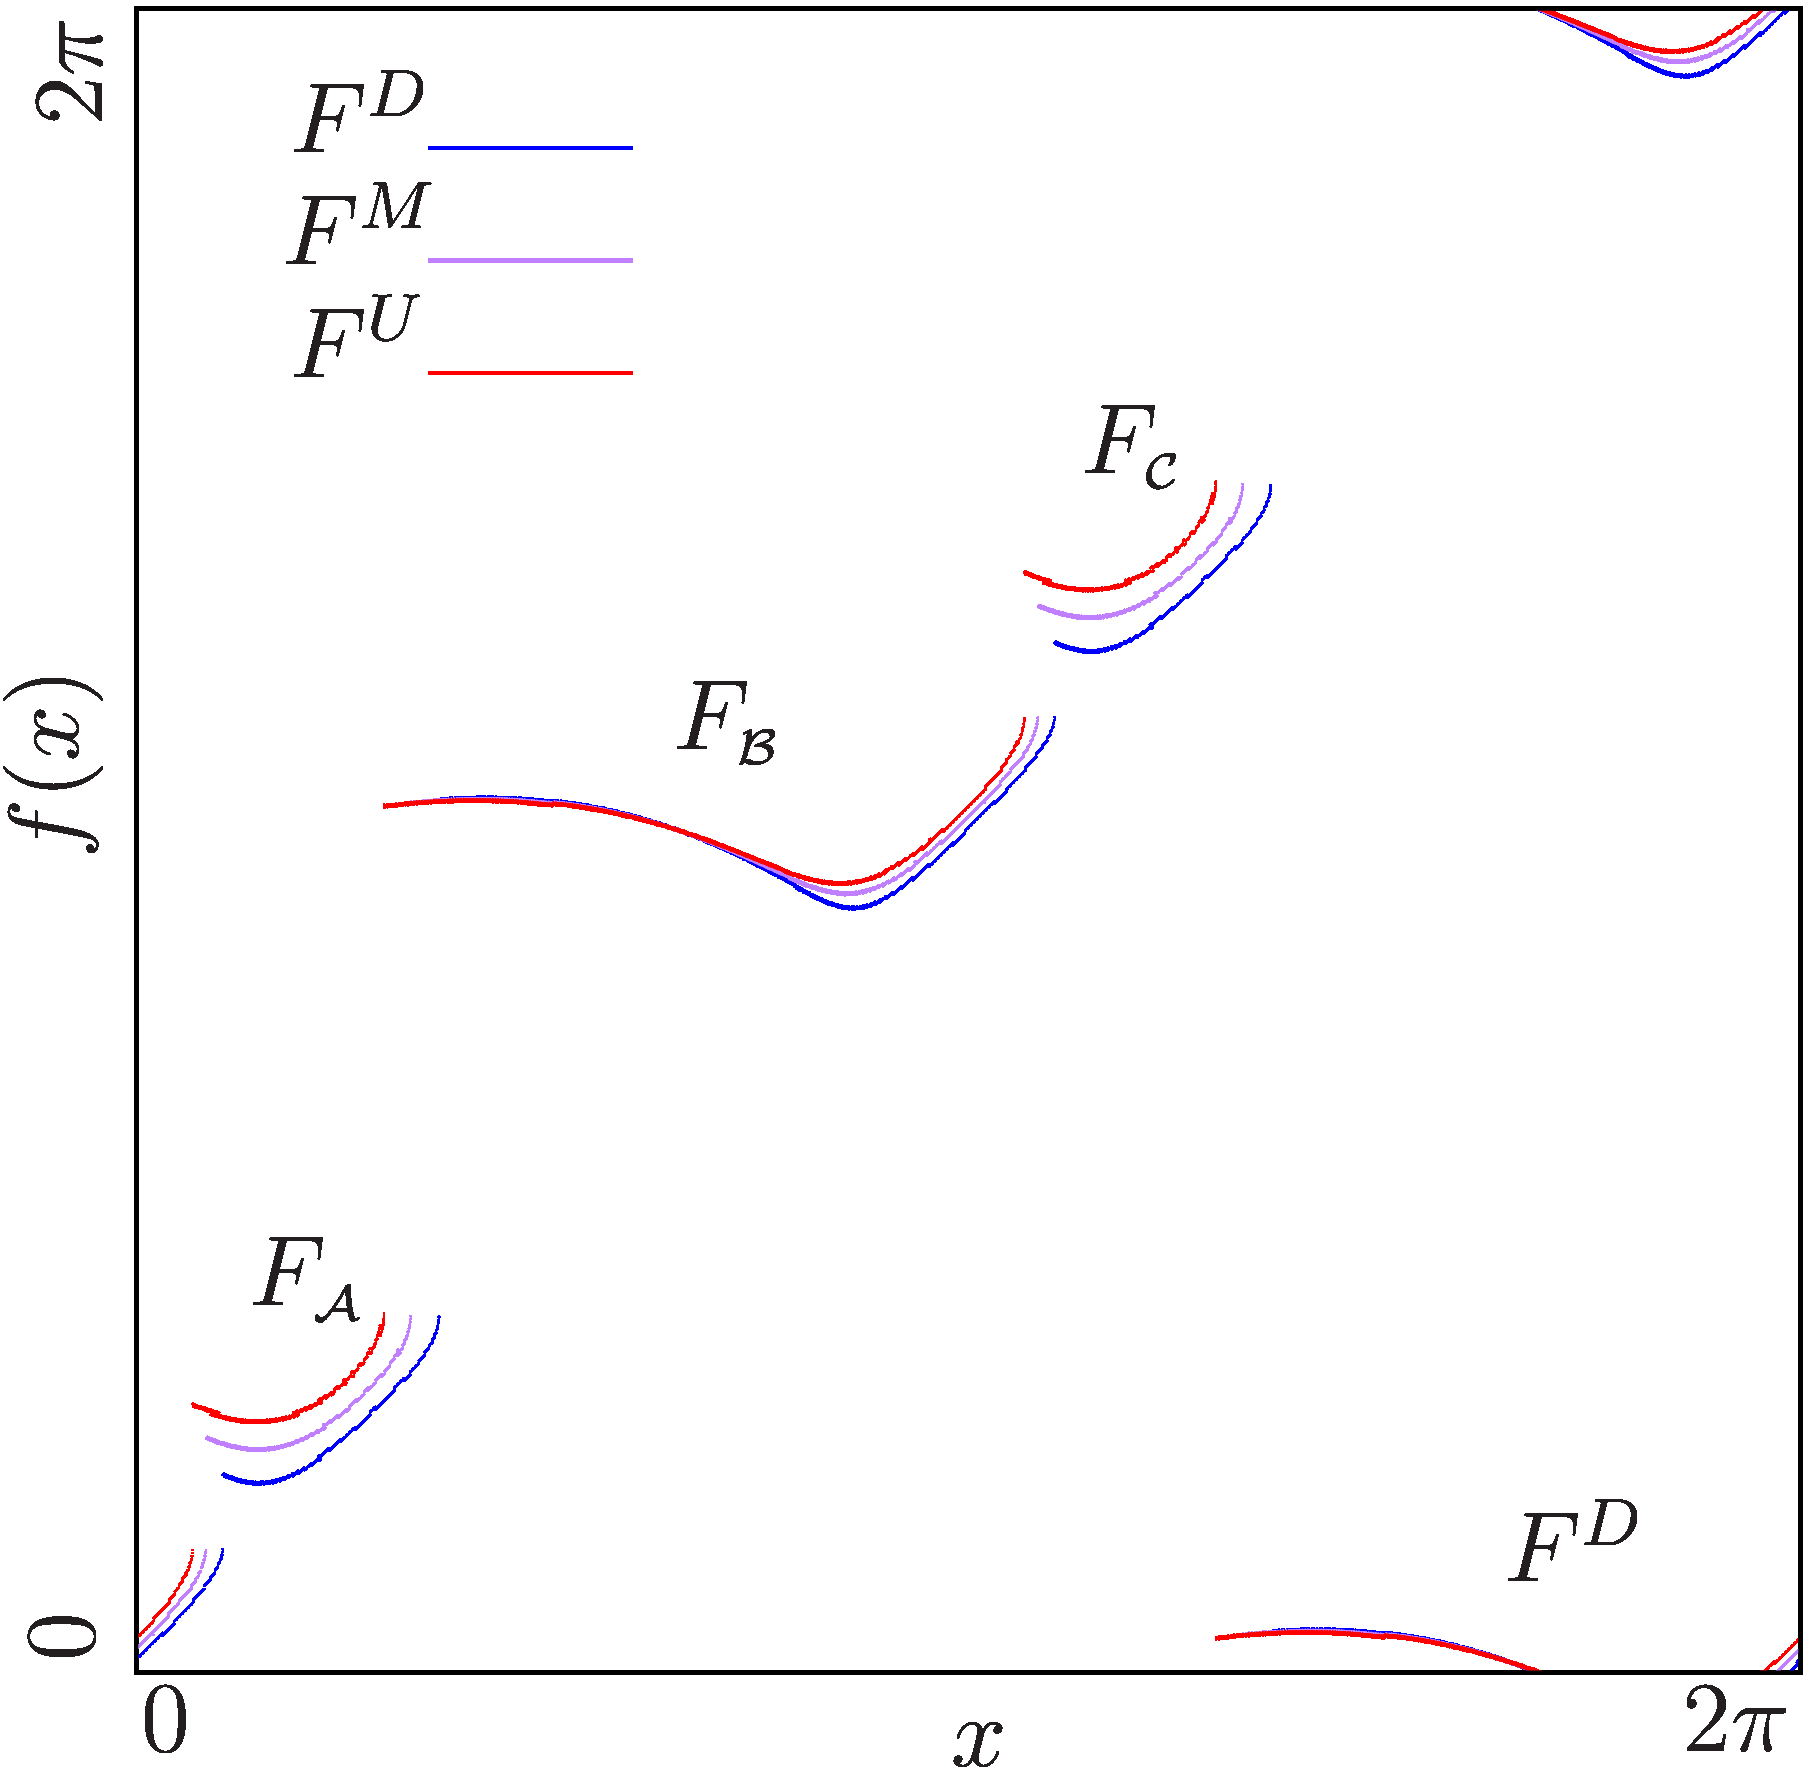
\includegraphics[width=.4 \textwidth]{../Figures/5/5.4b/illustration.png}
		\label{fig:setup.char.evolution.hi}
	}
	\caption[The isolated effects of the parameters on the original model function]{
		The isolated effects of the parameters $E_0$ and $\chi_0$ on the original model function.
		The parameter values used for plotting the functions are marked with points in \Cref{fig:setup.char.evolution.single.map}.
		(a) shows the evolution of the shape of the model function for different parameter values of $E_0$ while $\chi_0 = 0.2$ is fixed.
		The function $F^L$ is the model function with the parameter values at the point $L$ where $E_0 = 15$,
		$F^M$ is at the point $M$ where $E_0 = 17$,
		and $F^R$ is at the point $R$ where $E_0 = 19$.
		(b) shows the evolution of the shape of the model function for different parameter values of $\chi_0$ while $E_0 = 17$ is fixed.
		The function $F^D$ is the model function with the parameter values at the point $D$ where $\chi_0 = 0.1$,
		$F^M$ is at the point $M$ where $\chi_0 = 0.2$,
		and $F^U$ is at the point $U$ where $\chi_0 = 0.3$.
	}
	\label{fig:setup.char.evolution.single}
\end{figure}

\subsection{Decomposition of Combined Effects}
\label{sec:yunus.param.effects.decomposition}

This section considers the decomposition of the combined parameter effects listed in \Cref{sec:setup.char.paramfx.combined} into the effects of the isolated parameter effects listed in \Cref{sec:setup.char.paramfx.individual} and traces each effect back to its cause.
This is important, because some of the isolated parameter effects cancel out when the parameters are both varied as we will see later in this section.
For this, this section introduces a notation for the effects.
The effect of the values on the left side of a branch changing is denoted $\AL$, for the right side it is $\AR$, and for the whole branch it is $\AW$
The subscript indicates, which branch the change affects, and the superscript indicates, whether the values get larger $+$ or smaller $-$.
The effect of changing a local minimum is denoted as $\AMi$.
The meaning of the subscript stays the same as above, but the superscript also can include $L$ for movement to the left and $R$ for movement to the right.
Finally, the effect of moving borders is denoted as $\AB$.
The subscript now includes the two symbols of branches to which the border belongs and the superscript now has only $L$ or $R$.
For brevity, one does not write redundant branch names, so changes happening to branch $F_\A$ are also happening to branch $F_\C$.
For borders, changes to the border between branches $F_\A$ and $F_\B$ are also happening to the border between branches $F_\C$ and $F_\D$ and so on.

\Cref{table:setup.char.paramfx} lists all observed effects along the chains of parameter regions associated with cycles of the same period and their decomposition into effects of the single parameters.
The first part of the table includes all major changes observed in \Cref{sec:setup.char.paramfx.combined}.
The second part includes the minor change one can observe of the borders between the branches $f_\B$ and $f_\C$ moving to the left.
The second part also includes the changes observed in \Cref{sec:setup.char.paramfx.individual} that cancel out.
From this table we can see that $E_0$ causes the effects on the branches $F_\B$ and $F_\D$, while $\chi_0$ causes the changes to the branches $F_\A$ and $F_\C$, as well as the minor movement of the borders between the branches $F_\B$ and $F_\C$.
Note again that the change to the border of branches $F_\B$ and $F_\C$ also applies for the border between branches $F_\D$ and $F_\A$.

% table in next section for better layout
